\documentclass{article}
\usepackage[T2A]{fontenc}
\usepackage[russian]{babel}
\usepackage[utf8]{inputenc}

%%%%%%%%%%%%%%%%%%%%%%%%%%%% ДОП.СИМВОЛЫ  %%%%%%%%%%%%%%%%%%%%%%%%%%%%%%%%
\usepackage{amsmath}
\usepackage{amssymb}
\usepackage{latexsym}
\usepackage{amsfonts}
\usepackage{extarrows}
\usepackage{braket}
\usepackage{MnSymbol}
\usepackage{mathtools}
\usepackage{commath}

\DeclarePairedDelimiter{\ceil}{\lceil}{\rceil}
\DeclarePairedDelimiter{\floor}{\lfloor}{\rfloor}
%%%%%%%%%%%%%%%%%%%%%%%%%%%%%%%%%%%%%%%%%%%%%%%%%%%%%%%%%%%%%%%%%%%%%%%

%%%%%%%%%%%%%%%%%%%%%%%%%%%%%  ГРАФИКА  %%%%%%%%%%%%%%%%%%%%%%%%%%%%%%%%
%Цвета:
\usepackage{color} 
\usepackage{xcolor}

%Картиночки:
\usepackage{graphicx}
\graphicspath{{pictures/}}
\DeclareGraphicsExtensions{.pdf,.png,.jpg}

%Встроенная графика 
\usepackage{tikz}
\usetikzlibrary{
    shapes.symbols,
    shapes.geometric,
    shadows,arrows.meta,
    graphs
}

\usepackage{flowchart}
%%%%%%%%%%%%%%%%%%%%%%%%%%%%%%%%%%%%%%%%%%%%%%%%%%%%%%%%%%%%%%%%%%%%%%%%

%%%%%%%%%%%%%%%%%%%%%%%%%%%%%% ВЕРСТКА 1 %%%%%%%%%%%%%%%%%%%%%%%%%%%%%%%%%
\usepackage[toc,page]{appendix}
\usepackage{hyperref}
\hypersetup{
    unicode=true,
    colorlinks=true,
    linktoc=all,  
    linkcolor=blue,
}
\usepackage{hhline}
\usepackage{subcaption}
\usepackage{float}
\usepackage{enumitem}
%%%%%%%%%%%%%%%%%%%%%%%%%%%%%%%%%%%%%%%%%%%%%%%%%%%%%%%%%%%%%%%%%%%%%%%%

%%%%%%%%%%%%%%%%%%%%%%%%%%%%%% ВЕРСТКА 2 %%%%%%%%%%%%%%%%%%%%%%%%%%%%%%%%%
% Шрифты - настройки по умолчанию.
\renewcommand{\rmdefault}{cmr}
\renewcommand{\sfdefault}{cmss}
\renewcommand{\ttdefault}{cmtt}

%Формат секции
\makeatletter
\renewcommand{\@seccntformat}[1]{}
\makeatother


%Пробел
\setlength{\parindent}{0pt}
\setlength{\parskip}{3pt}

%Размеры страницы (не забыть подогнать под принтер)
\usepackage[left=2cm,right=2cm,bottom=2cm]{geometry}

%Списки:
\setlist{topsep=1pt, itemsep=0em}
%%%%%%%%%%%%%%%%%%%%%%%%%%%%%%%%%%%%%%%%%%%%%%%%%%%%%%%%%%%%%%%%%%%%%%%%%%%%%%%%%%%%%%%%%%%%

\title{Отчет по домашней работе по KNN}
\author{Михаил Михайлов, Ельцов Даниил}
\date{10 ноября 2020 г.}
\begin{document}
\maketitle
\tableofcontents

\section*{Резюме}
Была получена классификация для Ирисов Фишера. 
\newpage

\section{Постановка задачи}
Используя алгоритм KNN получить классификацию для ирисов Фишера.

\section{Используемый датасет}
\href{https://www.kaggle.com/uciёml/iris}{датасет}

\section{Описание решения}

Для обучения бралась случайная четвертая часть выборки и рассмтаривались 3 ближайших соседа. Число соседей было подообрано экспериментальным путем:


\section{Результаты}
Полученно разбиение на классы с точностью порядка 95\%. Такая точность достигается в том числе, за счет хорошего датасета. 

\begin{figure}[h!]
    \centering
    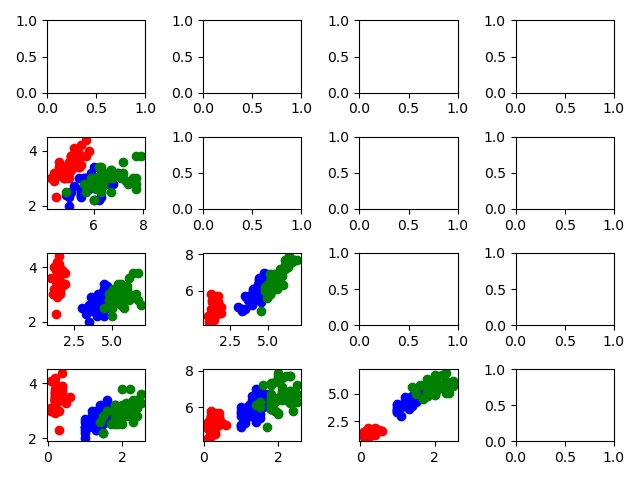
\includegraphics[scale=0.3]{results.jpg}
    \caption{Получившиеся классы. Графики представлены по каждой из четырех пар параметров \((i, j)\) в используемом датасете}
    \label{fig1}
\end{figure}

И

\begin{itemize}
    \item Код - Данил Ельцов
    \item Отчет - Михаил Михайлов
\end{itemize}

\end{document}

